\section{Windsimulation}
\label{sec:implementation_wind}

\subsection{Einleitung}

In diesem Abschnitt wird die Umsetzung der Windsimulation
vorgestellt. Da dieser Teil der Implementierung nicht mit der
Darstellung zusammenhängt, wird nur OpenCL verwendet. Der Abschnitt
knüpft direkt an \cref{sec:stam} an.

Zuerst wird die Wahl der Datenstrukturen besprochen. Es kommt hier
darauf an, eine möglichst performante Struktur zu wählen, die optimale
Zugriffszeiten liefert. Danach wird das Verfahren von Stam in
OpenCL-Code übertragen, dessen Bestandteile detailliert erläutert
werden.

Schließlich wird besprochen, wie die Hindernisse in die
Simulation eingespeist werden.

\subsection{Allgemeines}

Für die Simulation des Winds ist es wichtig, eine gute Datenstruktur
zur Speicherung der verwendeten Felder zu verwenden, um die
Speicherzugriffszeiten zu minimieren.

Wie bereits angesprochen bietet OpenCL zur Speicherung die Wahl
zwischen buffer objects und image objects (sofern image objects auf der
Zielplattform unterstützt werden). Beide Speicherarten haben leicht
unterschiedliche Anwendungsgebiete, daher müssen erst die
Anforderungen erarbeitet werden, die man an die Datenstruktur
stellt.

In vielen Kerneln ist man daran interessiert, den Wert für die
\PimiddyQuotes{aktuelle} Zelle im Gitter sowie den Wert aller
Nachbarzellen zu bestimmen. Der \PimiddyQuotes{Wert} kann je nach
betrachtetem Feldtyp entweder Druck, Geschwindigkeit oder etwas
anderes bedeuten. Bei der Advektion wird außerdem linear zwischen den
Voxeln in einer Nachbarschaft \emph{interpoliert}.

\begin{figure}[h]
\centering
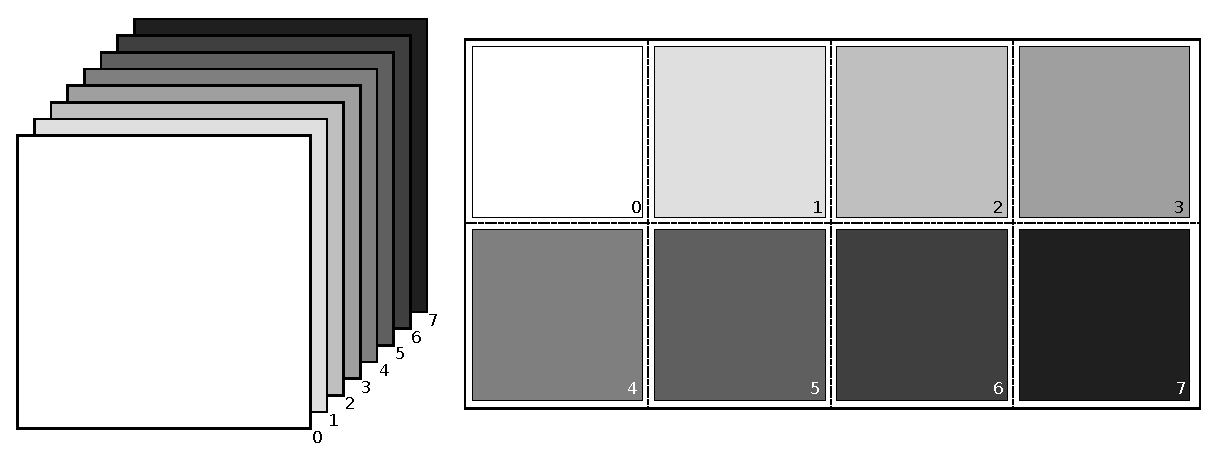
\includegraphics[width=14cm]{images/flat_texture}
\caption{Veranschaulichung einer Flat-3D-Textur}
\label{fig:implementation_flat_3d_texture}
\end{figure}

Schnelle Zugriffe auf einen Voxel samt seiner Nachbarn sind ein
Performancemerkmal von image objects. Sie würden sich daher für viele Kernel
anbieten, und viele GPU-Implementierungen von
strömungsmechanischen Verfahren nutzen in der Tat image objects (wenn auch
oft aus historischen Gründen). Allerdings ist das Schreiben von
3D-Texturen in OpenCL-1.1 nur mit einer Extension möglich. Als
Hilfsmaßnahme greift man hier üblicherweise zu sogenannten
\PimiddyBegriff{Flat-3D-Texturen} (\cite{Harris2003}). Hier werden die
einzelnen \PimiddyQuotes{Scheiben} der dreidimensionalen Struktur
nebeneinander in eine zweidimensionale Textur geschrieben, siehe
\cref{fig:implementation_flat_3d_texture}. Für die Umrechnung
zwischen 3D- und 2D-Koordinaten ist etwas Rechenaufwand
nötig. 2D-Texturen erlauben außerdem natürlicherweise nur
zweidimensionale Interpolation zwischen den Zellen. Benötigt man
hingegen dreidimensionale Interpolation, ist auch hier etwas
Mehraufwand zu verrechnen.

Image objects werden in einer optimierten Weise gespeichert, sodass
Leseoperationen beschleunigt werden
(\cite{Pharr:2005:GGP:1062395}). Diese optimierte Speicherung führt
aber dazu, dass das Schreiben in Texturen relativ langsam ist. Selbst
durchgeführte Benchmarks zeigen, dass buffer objects sogar im
Zweidimensionalen schneller sind als image objects. Daher wurden image
objects als mögliche Speicherform verworfen und es wurden einzig
Buffer verwendet. Diese erweisen sich außerdem als kompatibler, denn
OpenCL-Implementierungen müssen image objects nicht unterstützen.

Da Buffer eindimensional sind, muss zwischen drei- und
eindimensionalen Koordinaten konvertiert werden. Sei $(x,y,z)$ eine
dreidimensionale Koordinate und seien $(w,h,d)$ die Dimensionen eines
Buffers (er enthält also $w \cdot h \cdot d$ Elemente). Dann erhält
man einen eindimensionalen Index $i$ mittels:
\begin{equation}
\label{eq:implementation_wind_3d_to_2d}
i = w \cdot h \cdot z + w \cdot y + x
\end{equation}
Umgekehrt erhält man die $(x,y,z)$-Koordinaten eines Index mittels
\begin{equation}
\begin{split}
x &= i \PimiddyModulo w \\
y &= (i / w) \PimiddyModulo h \\
z &= i / (w \cdot h)  \\
\end{split}
\end{equation}
Im Folgenden wird das Verfahren von Stam in OpenCL umgesetzt. Fast
alle Kernel greifen hierbei auf den Buffer zurück, der die
Hindernisinformationen enthält. Im letzten Abschnitt wird erklärt, wie
dieser Buffer gefüllt wird.

\subsection{Verfahren nach Stam in OpenCL}

\subsubsection{Allgemeines}
\label{sec:implementation_wind_stam_general}

Es sollen nun die einzelnen Schritte des Verfahrens in OpenCL-Kernel
umgewandelt werden. Der Teil des Programms, der auf dem Host läuft,
soll hier nicht in Gänze erarbeitet werden. Stattdessen soll deutlich
werden, in welcher Reihenfolge die Kernel aufgerufen werden und welche
Daten beim Aufruf gelesen und geschrieben werden. Aus
Einrückungsgründen werden einige Bezeichner abgekürzt, aber immer so,
dass aus der Erläuterung \Pimiddybzw{} den Kommentaren noch hervorgeht, was
sich dahinter verbirgt.

Die Simulation benötigt einige persistente Daten, also solche, die
zwischen den Simulationsschritten beibehalten werden und nicht nur
temporär für Berechnungen verwendet werden:

\begin{itemize}
\item ein Buffer \PimiddyInlineCode{boundaries} vom Typ
\PimiddyInlineCode{float}, der 1.0 enthält, wenn die zugehörige
Gitterzelle ein Hindernis enthält und 0.0 wenn nicht. Das Befüllen
dieses Buffers wird in
\cref{sec:implementation_wind_boundaries} beschrieben.
\item ein Buffer \PimiddyInlineCode{velocity} vom Typ
\PimiddyInlineCode{float3}, der das aktuelle Geschwindigkeitsfeld enthält.
Dieses Feld wird anfangs auf $(0,0,0)$ gesetzt. Der Wind wird manuell von
einer Seite in die Simulation gespeist (siehe
\cref{sec:implementaion_wind_in_outflow}) und breitet sich dann
aus.
\item Viele der Algorithmen benötigen außerdem das aktuelle
\PimiddyQuotes{Zeitdelta} \PimiddyInlineCode{float dt}. Es gibt die
Zeit an, die seit dem letzten Simulationsdurchlauf vergangen ist. Mit
Hilfe dieser Größe wird die Simulation zeitlich normiert. Lange
Zeitabstände zwischen den diskreten Frames sollen zu größeren
Veränderungen im Windfeld führen.
\end{itemize}

Die meisten Kernel werden mit einer dreidimensionalen Arbeitsgröße
initialisiert, die der Größe des Gitters entspricht. Ein Work-Item
erhält also einen dreidimensionalen Vektor als globale ID, welcher die
Gitterposition angibt, die das Work-Item bearbeiten soll.

Da die buffer objects mit den Feldern allerdings eindimensional sind,
bietet es sich an, den Übergang von einem drei- zu einem
eindimensionalen Index in eine Funktion auszulagern. Diese Funktion
kann gleichzeitig testen, ob die gegebene Position den Rand des
Gitters verlässt, und in dem Fall den nächstgelegenen Voxel am Rand
zurückliefern. So lassen sich auf einfache Weise alle Nachbarn eines
Voxels aus dem Buffer extrahieren.

Die Funktion \PimiddyInlineCode{i4p} ist im Folgenden
dargestellt\PimiddyTodo{Das \PimiddyInlineCode{uint} wird nicht
highlighted}:

\begin{minted}[frame=lines,mathescape]{opencl}
// Bekommt die Gittergroesse s und eine 3D-Position p.
// Liefert einen Index.
uint i4p(uint3 p,uint3 s)
{
    // Komponentenweise in gueltigen
    // Bereich $[0,n-1]$ transformieren
    p = clamp(
        p,
        (uint3)(0),
        s - 1);

    return s.w * s.h * p.z + s.w * p.y + p.x;
}
\end{minted}

Für die Indextransformation wurde
\cref{eq:implementation_wind_3d_to_2d} verwendet.  Die
Standardbibliotheksfunktion \PimiddyInlineCode{clamp} stellt sicher,
dass ein Wert innerhalb eines Intervalls bleibt:
\begin{align}
\PimiddyFormelText{clamp}(x,a,b) = \max \{ a,\min \{ b,x \} \}
\end{align}

\subsubsection{Advektion}
\label{sec:implementation_wind_advection}

\begin{figure}
	\begin{subfigure}[t]{0.5\textwidth}
		\centering
		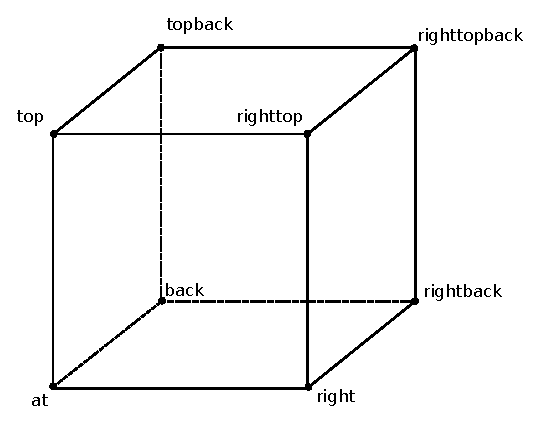
\includegraphics[width=\textwidth]{images/right_neighborhood}
                \caption{Veranschaulichung der Nachbarschaftsstruktur \PimiddyInlineCode{neighbors}.}
\label{fig:implementation_right_neighbors}
	\end{subfigure}
    ~
	\begin{subfigure}[t]{0.5\textwidth}
		\centering
		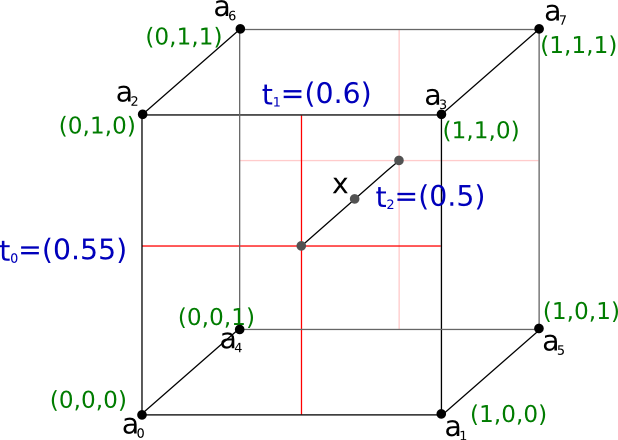
\includegraphics[width=\textwidth]{images/ndinterpolation}
		\caption{Dreidimensionale Interpolation mit dem Beispielvektor $(0.55,0.6,0.0.5)$}
\label{fig:implementation_wind_interpolation}
	\end{subfigure}
	\caption{Die dreidimensionale Nachbarschaft \PimiddyInlineCode{neighbors}}
\end{figure}

Der erste Schritt im Verfahren von Stam ist die Advektion des
Vektorfeldes \PimiddyInlineCode{velocity}
(\Pimiddyvgl{} \cref{sec:stam_advection}). Der dazugehörige Kernel ist in
mehrere Funktionen und Strukturen aufgeteilt, die nun im einzelnen
erklärt werden.

Vom aktuellen Voxel aus verfolgt man den Geschwindigkeitsvektor in
\PimiddyInlineCode{velocity} zurück und landet dabei, weil der
Vektor aus Fließkommawerten besteht, im Allgemeinen zwischen 8
Gitterzellen. Diese 8 Zellen nutzt man für eine lineare Interpolation,
um die neue Geschwindigkeit zu finden. Es bietet sich an, zunächst
eine Struktur zu definieren, um einen Geschwindigkeitswert sowie die
direkten Nachbarn zu speichern (siehe
\cref{fig:implementation_right_neighbors}).

\begin{minted}[frame=lines]{c}
typedef struct
{
    float3 at;
    float3 right,top,back,righttop;
    float3 rightback,topback;
    float3 righttopback;
} neighbors;
\end{minted}

Eine Instanz dieser Struktur wird von der zugehörigen Funktion
\PimiddyInlineCode{neighbors\_for\_pos} zurückgegeben, die eine
beliebige (diskrete) Position im Gitter sowie die Größe des Gitters
als Eingabe erhält. Die Funktion greift auf \PimiddyInlineCode{i4p}
zurück und ist so gegen Zugriffe außerhalb des Gitters geschützt:

\begin{minted}[frame=lines]{c}
// Parameter genau wie i4p, zusaetzlich noch "b"
neighbors neighbors_for_pos(
    global float3 *b,
    uint3 p,
    uint3 s)
{
    neighbors result;
    result.at = b[i4p(p,s)];
    result.right = b[i4p(p+(uint3)(1,0,0),s)];
    result.top = b[i4p(p+(uint3)(0,1,0),s)];
    result.back = b[i4p(p+(uint3)(0,0,1),s)];
    result.righttop = b[i4p(p+(uint3)(0,1,1),s)];
    result.rightback = b[i4p(p+(uint3)(1,0,1),s)];
    result.topback = b[i4p(p+(uint3)(0,1,1),s)];
    result.righttopback = b[i4p(p+(uint3)(1,1,1),s)];
    return result;
}
\end{minted}

Mit Hilfe einer Instanz von \PimiddyInlineCode{neighbors} und einem
beliebigen Vektor im Einheitsintervall ${[0,1]}^3$ soll ein
interpolierter Vektor erzeugt werden. Hier hilft die OpenCL-C-Funktion
\PimiddyInlineCode{mix}, die linear zwischen zwei Werten anhand eines
dritten Wertes interpoliert:
\begin{align}
\PimiddyFormelText{mix}(a,b,x) = (1-x)\cdot a + x \cdot b
\end{align}
Diese Funktion wird speziell auf Grafikkarten in hocheffektiven Code
übersetzt, da sie sich auf sogenannte
\PimiddyQuotes{multiply-add-Operationen} (auch
\PimiddyQuotes{MAD} genannt) zurückführen lässt. Darunter versteht man
skalare Operationen der Form $a\cdot x + b$, also eine Multiplikation
gefolgt von einer Addition. Da dies in der Grafikpipeline häufig
auftritt, sind die Arithmetikchips einer GPU speziell darauf
ausgelegt. Auf \PimiddyInlineCode{mix} wird in der unten stehenden
\PimiddyInlineCode{interpolate\_neighbors} mehrfach zurückgegriffen:

\begin{minted}[frame=lines,mathescape]{c}
float3 interpolate_neighbors(
    neighbors n,
    // v ist ein Vektor im Intervall $[0,1]^3$
    float3 v)
{
    float3
        v1 = mix(
            mix(n.at, n.right, v.x),
            mix (n.top, n.righttop, v.x),
            v.y),
        v2 = mix(
            mix(n.back, n.rightback, v.x),
            mix(n.topback, n. righttopback, v.x),
            v.y);

    return mix(v1,v2,v.z);
}
\end{minted}

Das Funktionsprinzip ist am Beispiel in
\cref{fig:implementation_wind_interpolation} verdeutlicht. Es wird
erst vier mal auf der $x$-Achse interpoliert, dann zwei mal auf der
$y$-Achse und schließlich einmal auf der $z$-Achse.

Der eigentliche Advektionskernel erhält als Eingabe ein quellenfreies
Geschwindigkeitsfeld \PimiddyInlineCode{input} und schreibt die
Ausgabe in das Feld \PimiddyInlineCode{output}:

\begin{minted}[frame=lines]{c}
kernel void advection(
    global float *boundary,
    global float3 *input,
    global float3 *output,
    // Das Zeitdelta
    float dt,
    // Gibt die Gittergroesse an
    uint3 size)
{
    uint3 position = (uint3)(
        get_global_id(0),
        get_global_id(1),
        get_global_id(2));

    uint index = i4p(position,size);

    if(boundary[index] != 0.0f)
    {
        output[index] = (float3)(0.0f);
        return;
    }

    float3
        v = input[index],
        // Konvertiere mit convert_float3 die diskrete Position
        // in eine Fliesskommaposition. Fuehre dann Advektion durch.
        advected = convert_float3(position) - dt * v,
        // fract liefert den Fliesskommateil eines Vektors.
        fractions = fract(advected_vector);

    neighbors n = neighbors_for_pos(
        input,
        position,
        size);

    output[index] = interpolate_neighbors(
        n,
        fractions);
}
\end{minted}

\subsubsection{In- und Outflow}
\label{sec:implementaion_wind_in_outflow}

Nach der Advektion werden die In- und Outflowboundaries behandelt
(\Pimiddyvgl{} \cref{sec:stam_boundaries}). Im Gegensatz zu den anderen
Kerneln wird hier nicht das gesamte Feld als globale Arbeitsgröße
gewählt, sondern nur eine Teilmenge des Gitters. Die Kernel sind so
einfach gehalten, dass sie hier nur erläutert, aber nicht im Code
vorgestellt werden.

Die Inflow-Boundaries gestalten sich sehr einfach. Es wird ein Vektor
vorgegeben, der die momentane Windstärke und -richtung angibt. Dann
wird eine Seite des Simulationswürfels mit diesem Vektor
gefüllt. Stams Verfahren sorgt dafür, dass sich der Wind langsam im
Simulationsbereich ausbreitet.

Bei den Outflow-Boundaries werden die 6 Randseiten des Würfels separat
behandelt. Jede Seite wird in die jeweils benachbarte
\PimiddyQuotes{Scheibe} kopiert; für die linke Seite in die Scheibe
rechts daneben, die Oberseite in die Scheibe einen drunter, und so
weiter.

\subsubsection{Projektion}
\label{sec:implementation_wind_projection}

\begin{figure}[ht]
\centering
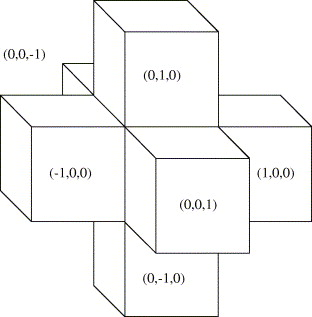
\includegraphics[width=6cm]{images/von_neumann}
\caption{Die dreidimensionale Von Neumann-Nachbarschaft}
\label{fig:implementation_wind_von_neumann_neighbors}
\end{figure}

Nach der Advektion ist das Vektorfeld $\vec{u}$ nicht mehr quellenfrei
und der Projektionsoperator muss angewendet werden
(\Pimiddyvgl{} \cref{sec:stam_projection}). Dazu bestimmt man zuerst die
Divergenz $\PimiddyDiv \vec{u}$ des Vektorfeldes und löst dann das
Gleichungssystem $\PimiddyLaplace x = \PimiddyDiv \vec{u}$ nach $x$
mit Hilfe des Jacobiverfahrens. Der Gradient von $x$ wird schließlich
von $\vec{u}$ subtrahiert und das Feld ist wieder quellenfrei.

Man benötigt also zunächst die Divergenz des Vektorfeldes. Analog zur
Advektion wird eine Struktur definiert, um die Von
Neumann-Nachbarschaft eines Gitterpunktes zu speichern (siehe
\cref{fig:implementation_wind_von_neumann_neighbors}):

\begin{minted}[frame=lines]{c}
typedef struct vn_neighbors
{
    float3 at;
    float3 left, right;
    float3 top, bottom;
    float3 front, back;
    float boundary_at;
    float boundary_left, boundary_right;
    float boundary_top, boundary_bottom;
    float boundary_front, boundary_back;
};
\end{minted}

Die Struktur enthält zusätzlich die zu den Nachbarn gehörigen
Hinderniswerte. Die Bestimmung dieser Werte und die der Vektoren
verläuft nach demselben Schema wie bei der Advektion und sei im
Folgenden ohne den zugehörigen Code mit
\PimiddyInlineCode{vn\_neighbors\_for\_pos(...)}  bezeichnet.

Bei der Bestimmung der Divergenz müssen die Randbedingungen beachtet
werden. Ist einer der Nachbarn des aktuellen Voxels von einem
Hindernis ausgefüllt, wird statt des Vektors an dieser Stelle der
\emph{Nullvektor} angenommen:
\begin{minted}[frame=lines]{c}
vn_neighbors n = vn_neighbors_for_pos(...);
if(n.boundary_left != 0.0f)
    n.left = (float3)(0.0f);
\end{minted}
Statt dies jedoch als eine \PimiddyInlineCode{if}-Bedingung
umzusetzen, wird stattdessen eine Multiplikation mit dem Randwert
verwendet.

Dies rührt daher, dass GPUs sich suboptimal verhalten, wenn mehrere
Work-Units in einer Work-Group unterschiedliche Ausführungspfade durch
den Code nehmen. Bei einer \PimiddyInlineCode{if}-Abfrage, die
beispielsweise für nur ein Work-Item \PimiddyInlineCode{true} ergibt,
durchlaufen dennoch \emph{alle} Work-Units der Work-Group den Rumpf
des \PimiddyInlineCode{if}-Statements, wobei die Ergebnisse der
\PimiddyQuotes{toten} Ausführungspfade verworfen werden. Natürlich
geschieht dies transparent für den Anwender, sodass keine
unerwünschten Nebeneffekte eintreten.

Die obige Abfrage lässt sich wie folgt umschreiben:

\begin{minted}[frame=lines]{c}
vn_neighbors n = vn_neighbors_for_pos(...);
n.left = (1.0f - n.boundary_left) * n.left;
\end{minted}

Hier liegt wieder eine MAD-Operation vor, der Code ist also wieder
sehr effizient.

Der zur Divergenz gehörige Kernel hat die folgende Form:

\begin{minted}[frame=lines]{c}
kernel void divergence(
    global float3 *input,
    global float *output,
    global float *boundary,
    uint3 size)
{
    uint3 position = (uint3)(
        get_global_id(0),
        get_global_id(1),
        get_global_id(2));

    uint index = i4p(position,size);

    vn_neighbors n = vn_neighbors_for_pos(
        input,
        position,
        boundary,
        size);

    float3 z = (float3)(0.0f);

    // Hier geschieht die Behandlung der Randbedingungen.
    // Es wird ausgenutzt, dass die Randwerte die Werte 0 oder 1
    // annehmen.
    n.left = mix(n.left, z, n.boundary_left);
    n.right = mix(n.right, z, n.boundary_right);
    n.top = mix(n.top, z, n.boundary_top);
    n.bottom = mix(n.bottom, z, n.boundary_bottom);
    n.front = mix(n.front, z, n.boundary_front);
    n.back = mix(n.back, z, n.boundary_back);

    // Da die Gittergroesse 1 betraegt, vereinfacht sich die Formel
    // aus dem ersten Abschnitt ein wenig.
    output[index] =
        (n.right - n.left).x +
        (n.bottom - n.top).y +
        (n.front - n.back).z;
}
\end{minted}

Um die Ähnlichkeit mit den restlichen Kerneln aufzuzeigen wurde hier
wieder die Funktion \PimiddyInlineCode{mix} verwendet.

Anschließend wird das Jacobiverfahren durchgeführt. Das
Verfahren ist iterativ, der Jacobi-Kernel muss also mehrfach gestartet
werden. Um Speicherplatz zu sparen, bietet sich ein
\PimiddyQuotes{Ping-Pong-Schema} an. Dazu werden zwei zusätzliche
buffer objects \PimiddyInlineCode{s1,s2} benötigt, welche jeweils ein
Skalarfeld speichern. Anfangs enthält \PimiddyInlineCode{s1} die
initiale Lösung für die Poissongleichung $\PimiddyLaplace x =
\PimiddyDiv \vec{u}$, also einfach das Nullfeld $x=0$. Eine Anwendung des
Jacobi-Kernels füllt \PimiddyInlineCode{s2} mit der ersten Iteration
des Verfahrens. Diese wird zur Eingabe der nächsten Iteration, die
\PimiddyInlineCode{s1} überschreibt, und so weiter. Nach gerade vielen
Iterationsschritten enthält \PimiddyInlineCode{s1} die endgültige
Lösung. \Cref{alg:implementation_wind_ping_ping} zeigt das
Verfahren im Pseudocode.

\begin{algorithm}
\caption{Der Ping-Pong-Algorithmus für das Jacobiverfahren}
\label{alg:implementation_wind_ping_ping}
\begin{algorithmic}
\Function{jacobi}{$\PimiddyDiv u$,b}
	\State s1 $\gets$ clCreateBuffer
	\State s2 $\gets$ clCreateBuffer
        \State fill\_buffer(s1,0)
        \State current\_source $\gets$ s1
        \State current\_destination $\gets$ s2
        \State clSetKernelArg(jacobi,0,$\PimiddyDiv u$)
        \State clSetKernelArg(jacobi,1,b)
        \For{i = 0; i < iterations; i++}
            \State clSetKernelArg(jacobi,2,current\_source)
            \State clSetKernelArg(jacobi,3,current\_destination)
            \State clEnqueueNDRangeKernel(jacobi)
            \State swap(current\_source,current\_destination)
        \EndFor
        \State \Return s1
\EndFunction
\end{algorithmic}
\end{algorithm}

Die Randbedingungen im Jacobi-Kernel werden ähnlich denen im
Divergenz-Kernel behandelt. Ist einer der Nachbarn von einem Hindernis
ausgefüllt, wird statt des Vektors an dieser Stelle der Vektor im
\emph{Zentrum der Nachbarschaft} angenommen. Dies lässt sich auch mit
der Operation \PimiddyInlineCode{mix} durchführen.

\begin{minted}[frame=lines]{c}
kernel void jacobi(
    global float *divergence,
    global float *boundary,
    global float3 *input,
    global float *output,
    uint3 size)
{
    uint3 position = (uint3)(
        get_global_id(0),
        get_global_id(1),
        get_global_id(2));

    uint index = i4p(position,size);

    vn_neighbors n = vn_neighbors_for_pos(
        input,
        position,
        boundary,
        size);

    n.left = mix(n.left, n.at, n.boundary_left);
    n.right = mix(n.right, n.at, n.boundary_right);
    n.top = mix(n.top, n.at, n.boundary_top);
    n.bottom = mix(n.bottom, n.at, n.boundary_bottom);
    n.front = mix(n.front, n.at, n.boundary_front);
    n.back = mix(n.back, n.at, n.boundary_back);

    float sum    = n.left + n.right + n.top + n.bottom + n.front + n.back,
          result = (sum - divergence[index]) / 6.0f;

    output[index] = mix(
        result,
        center,
        1.0f/3.0f);
}

\end{minted}

Der Code zeigt die gewichtete Jacobi-Iteration mit Wichtungswert
$\frac{1}{3}$, der sich als günstig herausgestellt hat.

Die Zahl der Iterationen kann von der Leistung der Grafikkarte
abhängig gemacht werden. Sie sollte jedoch mindestens 20
betragen. Gute Ergebnisse werden bei 40 Iterationen
erzielt.

Die Berechnung des Gradienten von $x$ und die darauf folgende
Subtraktion von $\vec{u}$ lässt sich (auch aus Performancegründen) in
einem einzigen Kernel behandeln. In diesem Kernel werden auch die vom
Jacobi-Verfahren nur unvollständig gelösten Randbedingungen
erzwungen. Der Kernel erfüllt folgende Aufgaben:

\begin{enumerate}
\item Er bestimmt den Gradienten des Druckfeldes. Es wird für einen
Nachbarwert wieder der Wert im Zentrum genommen, falls die
Nachbarzelle von einem Hindernis ausgefüllt ist.
\item Der Gradient wird vom Geschwindigkeitsfeld abgezogen.
\item Die free-slip-Randbedingungen werden erzwungen.
\end{enumerate}

\begin{figure}[h]
\centering
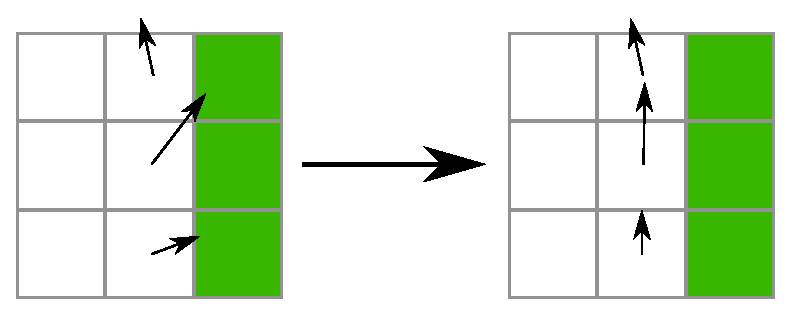
\includegraphics[width=10cm]{images/force_free_slip}
\caption{Die Korrektur der nach dem Projektionsschritt eventuell noch unvollständig gelösten Randbedingungen. Die markierten Felder enthalten Hindernisse, die $x$-Komponente der Geschwindigkeit wird daher auf $0$ gesetzt.}
\label{fig:implementation_wind_enforce_free_slip}
\end{figure}

In Schritt 3 wird für jede Koordinatenachse gespeichert, ob sich in
der Von Neumann-Nachbarschaft auf der Achse ein Hindernis
befindet. Ist dies der Fall, wird die Geschwindigkeitskomponente auf
dieser Achse auf 0
gesetzt. \Cref{fig:implementation_wind_enforce_free_slip}
verdeutlicht das Prinzip. Der Koeffizient, der die entsprechende
Komponente entweder behält oder gleich 0 setzt, kann als Funktion der
beiden Randwerte auf der Achse ausgedrückt werden:
\begin{minted}[frame=lines]{c}
float boundary_mask(float boundary_left,float boundary_right)
{
  return 1.0f - min(1.0f, boundary_left + boundary_right);
}
\end{minted}
Offenbar ist die Funktion genau dann $0$, wenn einer der beiden Werte
0 ist. Die Funktion enthält zudem keine (expliziten) bedingten
Anweisungen. Der gesamte Kernel ergibt sich wie folgt:
\begin{minted}[frame=lines]{c}
kernel void subtract_pressure_gradient(
    global float3 *velocity,
    global float *boundary,
    global float *pressure,
    uint3 size)
{
    // Schritt 1: Bestimmte Gradient des Druckfeldes
    uint3 position = (uint3)(
        get_global_id(0),
        get_global_id(1),
        get_global_id(2));

    uint index = i4p(position,size);

    vn_neighbors n = vn_neighbors_for_pos(
        input,
        position,
        boundary,
        size);

    if(boundary[index] == 1.0f)
    {
        velocity[current_index] =
            (float3)(
                0.0f,
                0.0f,
                0.0f);
        return;
    }

    float const center =
        pressure[index];

    // Bei Hinderniszellen wird das Zentrum gewaehlt
    n.left = mix(n.left, n.at, n.boundary_left);
    n.right = mix(n.right, n.at, n.boundary_right);
    n.top = mix(n.top, n.at, n.boundary_top);
    n.bottom = mix(n.bottom, n.at, n.boundary_bottom);
    n.front = mix(n.front, n.at, n.boundary_front);
    n.back = mix(n.back, n.at, n.boundary_back);

    float3 const pressure_gradient =
        (float3)(
            n.right.x - n.left.x,
            n.bottom.y - n.top.y,
            n.front.z - n.back.z);

    // Schritt 2 und 3: Gradient subtrahieren und Randbedingungen erzwingen
    float3 const vmask =
        (float3)(
            boundary_mask(n.boundary_left,n.boundary_right),
            boundary_mask(n.boundary_top,n.boundary_bottom),
            boundary_mask(n.boundary_front,n.boundary_back));

    velocity[current_index] =
        vmask * (velocity[index] - pressure_gradient);
}
\end{minted}

Das so erzeugte \PimiddyInlineCode{velocity}-Feld kann in der nächsten
Iteration wieder in die Advektionsroutine gegeben werden.
